
\chapter{E-Value: Evidence for Causation in Observational Studies with Unmeasured Confounding}
\chaptermark{E-Value}\label{chapter::evalue}


All the methods discussed in Part \ref{part::observational-studies}  rely crucially on the ignorability assumption. They require controlling for all confounding between the treatment and outcome. However, we cannot use the data to validate the ignorability assumption. Observational studies are often criticized due to the possibility of unmeasured confounding. The famous Yule--Simpson Paradox reviewed in Chapter \ref{chapter::correlationassociation} demonstrates that an unmeasured binary confounder can completely overturn an observed association between the treatment and outcome. However, to overturn a larger observed association, this unmeasured confounder must have a stronger association with the treatment and the outcome. In other words, not all observational studies are created equal. Some provide stronger evidence for causation than others. 


The following three chapters will discuss various sensitivity analysis techniques that can quantify the evidence of causation based on observational studies in the presence of unmeasured confounding. This chapter starts with the E-value, introduced by \citet{vanderweele2017sensitivity} based on the theory in \citet{ding2016sensitivity}. It is more useful for observational studies using logistic regressions to estimate the conditional risk ratio of a treatment on a binary outcome. Chapter \ref{chapter::sensitivity-ACE} discusses sensitivity analysis for the average causal effect based on outcome regression,  IPW, and doubly robust estimation.  Chapter \ref{sec::rosenbaum-sensitivity-analysis} discusses Rosenbaum's framework for sensitivity analysis for matched observational studies. 






\section{Cornfield-type sensitivity analysis}

Although we do not assume ignorability given $X$:
$$
Z\nind \{  Y(1), Y(0) \} \mid X ,
$$
we still assume latent ignorability given $X$ and an unmeasured confounder $U$: 
$$
Z\ind \{  Y(1), Y(0) \} \mid (X, U) . 
$$
The technique in this chapter works the best for a binary outcome $Y$ although it can be extended to other non-negative outcomes \citep{ding2016sensitivity}. Focus on binary $Y$ now. The true conditional causal effect on the risk ratio scale is defined as 
$$
\RR_{ZY\mid x}^\true = \frac{  \pr\{ Y(1) = 1\mid X=x  \} }{ \pr\{ Y(0) = 1\mid X=x  \} },
$$
and the observed conditional risk ratio equals 
$$
\RR_{ZY\mid x}^\obs = \frac{  \pr( Y  = 1\mid Z=1, X=x  ) }{ \pr( Y  = 1\mid  Z=0, X=x  ) }.
$$
In general, with an unmeasured confounder $U$,  they are different:
$$
\RR_{ZY\mid x}^\true  \neq \RR_{ZY\mid x}^\obs 
$$ 
because
$$
\RR_{ZY\mid x}^\true = \frac{  \int  \pr( Y = 1\mid Z=1, X=x, U=u  )  f(u \mid X=x) \diff u }
{ \int \pr( Y = 1\mid Z=0,  X=x , U=u  )  f(u \mid X=x) \diff u }
$$
and
$$
\RR_{ZY\mid x}^\obs = \frac{ \int   \pr( Y  = 1\mid Z=1, X=x , U=u ) f(u \mid Z=1, X=x) \diff u   }
{ \int  \pr( Y  = 1\mid  Z=0, X=x, U=u  ) f(u \mid Z=0, X=x) \diff u  } 
$$
are averaged over different distributions of $U$. 


Historically,  \citet{doll1950smoking} found that the risk ratio of cigarette smoking on lung cancer was $9$ even after adjusting for many observed covariates $X$\footnote{Their original analysis was based on a case-control study and estimated the odds ratio of cigarette smoking on lung cancer. But the risk ratio is close to the odds ratio since lung cancer is a rare outcome; see Proposition \ref{prop::2x2-independence}.}. \citet{Fisher::1957} criticized their result to be noncausal because it is possible that a hidden gene simultaneously causes cigarette smoking and lung cancer although the true causal effect of cigarette smoking on lung cancer is absent. This is the {\it common cause} hypothesis, also discussed by \citet{reichenbach1991direction}. \citet{Cornfield::1959} took a more constructive perspective and asked: how strong this unmeasured confounder must be to explain away the observed association between cigarette smoking and lung cancer? Below we will use  \citet{ding2016sensitivity}'s general formulation of the problem. 


Consider the following causal diagram:
$$
\xymatrix{
 &U \ar[dl] \ar[dr] \\
 Z   && Y 
}
$$
which conditions on $X$. So $Z\ind Y\mid (X, U)$. Conditioning on $X$ and $U$, we observe no association between $Z$ and $Y$; but conditioning on only $X$, we observe an association between $Z$ and $Y$.  Although we can allow $U$ to be general as \citet{ding2016sensitivity}, we assume that $U$ is binary to simplify the presentation. 


Define two sensitivity parameters:
$$
\RR_{ZU\mid x} = \frac{ \pr(U=1\mid Z=1,X=x) }{ \pr(U=1\mid Z=0,X=x)  } 
%\equiv \frac{  f_{1,x} }{  f_{0,x} }
$$
measures the treatment-confounder association, 
and
$$
\RR_{UY\mid x} = \frac{  \pr(Y=1\mid U=1, X=x) }{  \pr(Y=1\mid U=0, X=x) },
$$
measures the confounder-outcome association, conditional on covariates $X=x$.  We can show the main result below.

\begin{theorem}\label{thm::bounding-factor}
Under $Z\ind Y\mid (X, U)$, assume 
\begin{equation}\label{eq::largerthan1-evalue}
\RR_{ZY\mid x}^\obs > 1, \quad
 \RR_{ZU\mid x} > 1,\quad 
 \RR_{UY\mid x} > 1.
\end{equation}
We have 
$$
\RR_{ZY\mid x}^\obs \leq \frac{ \RR_{ZU\mid x}  \RR_{UY\mid x} }{  \RR_{ZU\mid x} + \RR_{UY\mid x} - 1} .
$$
\end{theorem}

In Theorem \ref{thm::bounding-factor}, we assume \eqref{eq::largerthan1-evalue}  without loss of generality. If $\RR_{ZY\mid x}^\obs < 1$, we can relabel the treatment and control levels to ensure $\RR_{ZY\mid x}^\obs > 1$. If $  \RR_{ZU\mid x}  < 1$, we can redefine the unmeasured confounder $U$ as $1-U$ to ensure $   \RR_{ZU\mid x}  > 1$. If $\RR_{ZY\mid x}^\obs > 1$ and $ \RR_{ZU\mid x} > 1$, then $ \RR_{UY\mid x}  > 1$ holds automatically. I relegate this subtle technical detail to Problem \ref{hw::technical-largerthan1}. 


Theorem \ref{thm::bounding-factor} shows the upper bound of the observed risk ratio of the treatment on the outcome if the conditional independence $Z\ind Y\mid (X, U)$ holds. Under this conditional independence assumption, the association between the treatment and the outcome is purely due to the association between the treatment and the confounder $\RR_{ZU\mid x} $, and the association between the confounder and the outcome, $\RR_{UY\mid x}$. The upper bound equals $\RR_{ZU\mid x} \times  \RR_{UY\mid x} /  (\RR_{ZU\mid x} + \RR_{UY\mid x} - 1)$. 
A similar inequality appeared in \citet{lee2011bounding}. 
It is also related to Cochran's formula or the omitted-variable bias formula for linear models, which was reviewed in Problem \ref{hw::cochran+ovb}.  



Reversely, to generate a certain value of the observed risk ratio $\RR_{ZY\mid x}^\obs$, the two confounding measures $\RR_{ZU\mid x} $ and $\RR_{UY\mid x}$ cannot be arbitrary. Their function $\RR_{ZU\mid x}  \times  \RR_{UY\mid x} /  (\RR_{ZU\mid x} + \RR_{UY\mid x} - 1)$ must be at least at large as $\RR_{ZY\mid x}^\obs$. 

I will give the proof of Theorem \ref{thm::bounding-factor}  below. 


\begin{myproof}{Theorem}{\ref{thm::bounding-factor}}
%For simplicity, we also write ``$X=x$'' as ``$x$'' in the conditional probabilities. 
%\frac{ \pr(U=1\mid Z=1,X=x) }{ \pr(U=1\mid Z=0,X=x)  } \equiv \frac{  f_{1,x} }{  f_{0,x} }
Define 
$$ 
f_{1,x} = \pr(U=1\mid Z=1,X=x),\quad
f_{0,x}  = \pr(U=1\mid Z=0,X=x) .
$$ 
We can decompose $\RR_{ZY\mid x}^\obs$ as
\begin{eqnarray*}
&&\RR_{ZY\mid x}^\obs  \\
&=& \frac{  \pr( Y  = 1\mid Z=1, X=x  ) }{ \pr( Y  = 1\mid  Z=0,  X=x  ) } \\
&=& \frac{ \left[ \splitfrac{ \pr(U=1\mid Z=1,  X=x) \pr( Y  = 1\mid Z=1, U=1,  X=x  ) }{+ \pr(U=0\mid Z=1,  X=x) \pr( Y  = 1\mid Z=1, U=0,  X=x  )} \right]}
{ \left[ \splitfrac{\pr(U=1\mid Z=0,  X=x) \pr( Y  = 1\mid  Z=0, U=1,  X=x  )}{  +  \pr(U=0\mid Z=0,  X=x) \pr( Y  = 1\mid  Z=0, U=0,  X=x  ) } \right]  } \\
&=& \frac{ \left[ \splitfrac{ \pr(U=1\mid Z=1,  X=x) \pr( Y  = 1\mid U=1,  X=x  ) }{+ \pr(U=0\mid Z=1,  X=x) \pr( Y  = 1\mid U=0,  X=x  )}\right] }
{  \left[ \splitfrac{ \pr(U=1\mid Z=0,  X=x) \pr( Y  = 1\mid   U=1,  X=x  )  }{+  \pr(U=0\mid Z=0,  X=x) \pr( Y  = 1\mid  U=0,  X=x  ) }\right]  } \\
&=& \frac{  f_{1,x} \RR_{UY\mid x} + 1- f_{1,x}  }{ f_{0,x} \RR_{UY\mid x} + 1- f_{0,x}  } \\
&=& \frac{  (\RR_{UY\mid x} - 1) f_{1,x} + 1  }{      \frac{  \RR_{UY\mid x} - 1}{  \RR_{ZU\mid x} }    f_{1,x} + 1  } .
\end{eqnarray*}
We can verify that $\RR_{ZY\mid x}^\obs$ is increasing in $f_{1,x} $ using the result in Problem \ref{hw::technical-for-evalue-increasing}. So letting $f_{1,x} = 1$, we have
$$
\RR_{ZY\mid x}^\obs \leq \frac{  (\RR_{UY\mid x} - 1) + 1  }{      \frac{  \RR_{UY\mid x} - 1}{  \RR_{ZU\mid x} }    + 1  }
= \frac{ \RR_{ZU\mid x}  \RR_{UY\mid x} }{  \RR_{ZU\mid x} + \RR_{UY\mid x} - 1} .
$$
\end{myproof}

In the proof of Theorem \ref{thm::bounding-factor}, we have obtain an identity
\begin{equation}
\label{eq::identity-evalue}
\RR_{ZY\mid x}^\obs = \frac{  (\RR_{UY\mid x} - 1) f_{1,x} + 1  }{      \frac{  \RR_{UY\mid x} - 1}{  \RR_{ZU\mid x} }    f_{1,x} + 1  } .
\end{equation}
But this identity involves three parameters 
$$
\{  f_{1,x}, \RR_{ZU\mid x},  \RR_{UY\mid x}  \} ;
$$
see Problem \ref{hw::Schlesselman1978formula} for a related formula. In contrast, the upper bound in Theorem \ref{thm::bounding-factor} involves only two parameters 
$$
\{  \RR_{ZU\mid x},  \RR_{UY\mid x}  \}
 $$
 which measure the strength of the confounder.
 Mathematically, the identity \ref{eq::identity-evalue} is stronger than the inequality in Theorem \ref{thm::bounding-factor}. However, \ref{eq::identity-evalue}  involves more sensitivity parameters compared with Theorem \ref{thm::bounding-factor}. Therefore, we face a trade-off of accuracy and convenience in sensitivity analysis.


\section{E-value}

Lemma \ref{lemma::betaw1w2} below is useful for deriving interesting corollaries of Theorem \ref{thm::bounding-factor}. I relegate its proof to Problem \ref{hw::proof-lemma-evalue}. 

\begin{lemma}
\label{lemma::betaw1w2}
Define $\beta(w_1, w_2) = w_1 w_2/(w_1 + w_2 - 1)$ for $w_1 > 1$ and $w_2 > 1$.  
\begin{enumerate}
[(1)]
\item
$\beta(w_1, w_2)$ is symmetric in $w_1$ and $w_2$;
\item
$\beta(w_1, w_2)$ is increasing in both $w_1$ and $w_2$;
\item\label{beta2}
$\beta(w_1, w_2) \leq w_1$ and $\beta(w_1, w_2) \leq w_2$;
\item\label{beta3}
$\beta(w_1, w_2) \leq w^2/(2w-1)$, where $w = \max(w_1, w_2)$.
\end{enumerate}
\end{lemma}



 


Using Theorem \ref{thm::bounding-factor} and Lemma \ref{lemma::betaw1w2}\eqref{beta2}, we have
$$
 \RR_{ZU\mid x} \geq \RR_{ZY\mid x}^\obs, \quad  \RR_{UY\mid x}  \geq \RR_{ZY\mid x}^\obs , 
$$
or, equivalently, 
$$
\min( \RR_{ZU\mid x} ,  \RR_{UY\mid x} ) \geq \RR_{ZY\mid x}^\obs.
$$
Therefore, to explain away the observed relative risk, both confounding measures $\RR_{ZU\mid x} $ and $  \RR_{UY\mid x}$ must be at least as large as $\RR_{ZY\mid x}^\obs$.
\citet{Cornfield::1959} first derived the inequality $\RR_{ZU\mid x} \geq \RR_{ZY\mid x}^\obs$, also called the {\it Cornfield inequality} \citep{gastwirth1998cornfield}. \citet{Schlesselman::1978} derived the inequality $\RR_{UY\mid x}  \geq \RR_{ZY\mid x}^\obs$. 
These are related to to the {\it data processing inequality} in information theory\footnote{In information theory, the {\it mutual information}  
$$
I(A,B) = \iint p(a,b) \log_2 \frac{  p(a,b) }{p(a)p(b)} \text{d} a \text{d} b
$$ 
measures the dependence between two random variables $A$ and $B$, where $p(\cdot)$ denotes the joint or marginal density of $(A,B)$. The {\it data processing inequality}  is a famous result: if $Z\ind Y \mid U$, then $I(Z,Y) \leq I(Z,U)$ and $I(Z,Y) \leq I(U,Y)$.
Lihua Lei and Bin Yu both pointed out to me the connection between Cornfield's inequality and the data processing inequality. 
}. 



If we define $w = \max( \RR_{ZU\mid x} ,  \RR_{UY\mid x} )$, then we can use Theorem \ref{thm::bounding-factor} and Lemma \ref{lemma::betaw1w2}\eqref{beta3} to obtain
\begin{eqnarray*}
&&w^2/(2w-1) \geq \beta( \RR_{ZU\mid x} , \RR_{UY\mid x}) \geq \RR_{ZY\mid x}^\obs \\ 
&\Longrightarrow & w^2 - 2 \RR_{ZY\mid x}^\obs w + \RR_{ZY\mid x}^\obs \geq 0,
\end{eqnarray*}
which is a quadratic inequality. One root $  \RR_{ZY\mid x}^\obs - \sqrt{ \RR_{ZY\mid x}^\obs (\RR_{ZY\mid x}^\obs - 1)} $ is always smaller than or equal to $1$, so we have
$$
w = \max( \RR_{ZU\mid x} ,  \RR_{UY\mid x} ) \geq \RR_{ZY\mid x}^\obs + \sqrt{ \RR_{ZY\mid x}^\obs (\RR_{ZY\mid x}^\obs - 1)} . 
$$
Therefore, to explain away the observed relative risk, the maximum of the confounding measures $\RR_{ZU\mid x} $ and $  \RR_{UY\mid x}$ must be at least as large as $\RR_{ZY\mid x}^\obs + \sqrt{ \RR_{ZY\mid x}^\obs (\RR_{ZY\mid x}^\obs - 1)} $.  
Based on this result, \citet{vanderweele2017sensitivity} introduced the following notion of  E-value for measuring the {\it evidence} of causation with observational studies. 

 


\begin{definition}
[E-Value]
With the observed conditional risk ratio $\RR_{ZY\mid x}^\obs$, define the E-Value as 
$$
\RR_{ZY\mid x}^\obs + \sqrt{ \RR_{ZY\mid x}^\obs (\RR_{ZY\mid x}^\obs - 1)} . 
$$ 
\end{definition}

 
 
The E-value is defined for the parameter  $\RR_{ZY\mid x}^\obs$. In practice, $\RR_{ZY\mid x}^\obs$ is estimated with sampling error. We can calculate the E-value based on the estimated $\RR_{ZY\mid x}^\obs$, as well as the corresponding E-values for the lower and upper confidence limits of $\RR_{ZY\mid x}^\obs$. 


Fisher's $p$-value measures the evidence for causal effects in randomized experiments. We have discussed the $p$-value based on the FRT in Part \ref{part::rcts} of this book. However, in observational studies with large sample sizes, $p$-values can be a poor measure of evidence for causal effects. Even if the true causal effects are $0$, a tiny amount of unmeasured confounding can bias the estimate, which can result in extremely small $p$-values given the small sampling uncertainty. The sampling uncertainty is usually secondary in observational studies with large sample sizes, but the uncertainty due to unmeasured confounding is often the first-order problem that does not diminish with increased sample sizes.  \citet{vanderweele2017sensitivity} argued that the E-value is a better measure of the evidence for causal effects in observational studies. 

 


\section{A classic example}
\label{sec::evalue-example}


I revisit a classic example below. 


\begin{example}\label{eg::hammond-evalue}
\citet{Hammond::1968} used the U.S. population to study the cigarette smoking and lung cancer relationship. Ignoring covariates, their data can be represented by a two-by-two table below:


\begin{center}
\begin{tabular}{ccc}
\hline 
 & Lung cancer & No lung cancer \\
 \hline 
 Smoker & 397 & 78557 \\
 Non-smoker & 51 & 108778  \\ 
 \hline 
\end{tabular}
\end{center} 


Based on the data, they obtained an estimate of the risk ratio $10.73$ with a 95\% confidence interval $[8.02, 14.36]$ (see Section \ref{section::asymptotic-inference-2x2} for the formulas). To explain away the point estimate, the E-value is 
$$
10.73 + \sqrt{10.73\times (10.73-1)} = 20.95;
$$
to explain away the lower confidence limit, the E-value is 
$$
8.02 +  \sqrt{8.02\times (8.02 - 1)} = 15.52.
$$

Figure \ref{fg::hammond-e-value} shows the joint values of the two confounding measures to explain away the point estimate and lower confidence limit of the risk ratio. In particular, to explain away the point estimate, they must lie in the area above the solid curve; to explain away the lower confidence limit, they must lie in the area above the dashed curve.\footnote{Based on some simple algebra, the solid curve and dashed curve are both hyperbolas.} 
\end{example}


The simple \ri{R} code below  computes the numbers in Example \ref{eg::hammond-evalue}:
 \begin{lstlisting}
> ## e-value based on RR
> evalue = function(rr)
+ {
+   rr + sqrt(rr*(rr - 1))
+ }
> 
> p1  = 397/(397+78557)
> p0  = 51/(51+108778)
> rr  = p1/p0
> logrr = log(p1/p0)
> se    = sqrt(1/397+1/51-1/(397+78557)-1/(51+108778))
> upper = exp(logrr+1.96*se)
> lower = exp(logrr-1.96*se)
> 
> ## point estimate
> rr
[1] 10.72978
> ## lower CI
> lower
[1] 8.017414
> ## e-value based on rr
> evalue(rr)
[1] 20.94733
> ## e-value based on lower CI
> evalue(lower)
[1] 15.51818
 \end{lstlisting}

\begin{figure}[t]
\centering
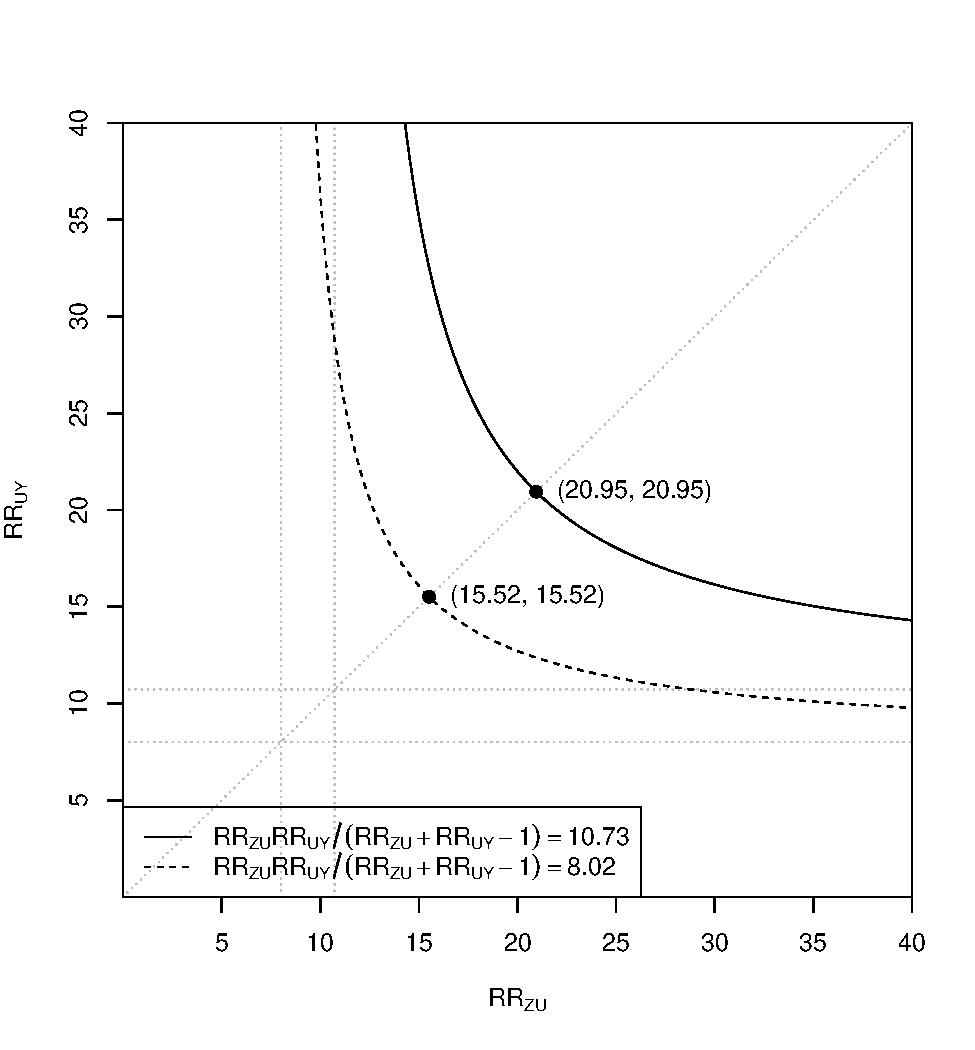
\includegraphics[width = 0.8 \textwidth]{figures/jointvalueplot.pdf}
\caption{Magnitude of confounding to explain away the observed risk ratio based on the data from \citet{Hammond::1968}}\label{fg::hammond-e-value}
\end{figure}



\section{Extensions}


\subsection{E-value and Bradford Hill's criteria for causation}

The E-value provides evidence for causation. But evidence is not a proof. With a larger E-value, we need a stronger unmeasured confounder to explain away the observed risk ratio; the evidence for causation is stronger. With a smaller E-value, we need a weaker unmeasured confounder to explain away the observed risk ratio; the evidence for causation is weaker. Coupled with the discussion in Section \ref{sec::evalue-monotone}, a larger observed risk ratio has stronger evidence for causation. This is closely related to Sir Bradford Hill's first criterion for causation: {\it strength} of the association \citep{hill1965environment}. Theorem \ref{thm::bounding-factor} provides a mathematical quantification of his heuristic argument. 


In a famous paper,  \citet{hill1965environment} proposed a set of nine criteria to provide evidence for causation between a presumed cause and outcome.


\begin{definition}\label{def::hill-causation}
Bradford Hill gave nine criteria for causation:
\begin{enumerate}
\item
strength;
\item
consistency;
\item
specificity;
\item
temporality;
\item
biological gradient;
\item
plausibility;
\item
coherence;
\item
experiment;
\item
analogy.
\end{enumerate}
\end{definition}


The E-value is a way to justify his first criterion. 
That is, stronger association often provides stronger evidence for causation because to explain away stronger association, we need stronger confounding measures. 
We have discussed randomized experiments in Part \ref{part::rcts}, which corroborates his eighth criterion. Due to the space limit, I omit the detailed discussion of his other criteria and encourage the readers to read  \citet{hill1965environment}. Recently, this paper has been re-printed as \citet{hill2020environment} with insightful comments from many leading researchers in causal inference. 




\subsection{E-value after logistic regression}

With a binary outcome, it is common for epidemiologists to use a logistic regression of the outcome $Y_i$ on the treatment indicator $Z_i$ and covariates $X_i$:
$$
\pr(Y_i = 1\mid Z_i, X_i) = \frac{  e^{\beta_0 + \beta_1 Z_i + \beta_2\tran X_i}  }{1  + e^{\beta_0 + \beta_1 Z_i + \beta_2\tran X_i}} .
$$
In the logistic model above, the coefficient of $Z_i$ is the log of the conditional odds ratio between the treatment and the outcome given the covariates:
$$
\beta_1 = \log \frac{   \pr(Y_i=1\mid Z_i =1, X_i=x)/  \pr(Y_i=0\mid Z_i =1, X_i=x)  }
{  \pr(Y_i=1\mid Z_i =0, X_i=x)/  \pr(Y_i=0\mid Z_i =0, X_i=x)  }  .
$$
Importantly, the logistic model assumes a common odds ratio across all values of the covariates. Moreover, when the outcome is rare in that $ \pr(Y_i=1\mid Z_i =1, X_i=x)$ and $\pr(Y_i=1\mid Z_i =0, X_i=x)$ are close to $0$, the conditional odds ratio approximates the conditional risk ratio (see Proposition \ref{prop::2x2-independence}(3)):
$$
\beta_1  \approx \log  \frac{   \pr(Y_i=1\mid Z_i =1, X_i=x)  }
{  \pr(Y_i=1\mid Z_i =0, X_i=x)  } = \log   \RR_{ZY\mid x}^\obs.
$$
Therefore, based on the estimated logistic regression coefficient and the corresponding confidence limits, we can calculate the E-value immediately. This is the leading application of the E-value. 




\begin{example}
\label{eg::NCHS2003}
The \ri{NCHS2003.txt} contains the National Center for Health Statistics birth certificate data, with the following binary indicator variables useful for us:


 

\begin{tabular}{ll}
\hline 
\texttt{PTbirth} &
 pre-term birth \\
\texttt{preeclampsia} &
 pre-eclampsia \\
\texttt{ageabove35}& 
 an older mother with age $\geq 35$ (the treatment) \\
\texttt{somecollege}&
 college education \\
\texttt{mar}& 
 marital status \\
\texttt{smoking}& 
 smoking status \\
\texttt{drinking}& 
 drinking status \\
\texttt{hispanic}& 
 mother's ethnicity  \\
\texttt{black}& 
 mother's ethnicity  \\
\texttt{nativeamerican}& 
 mother's ethnicity \\
\texttt{asian}& 
 mother's ethnicity\\
 \hline 
\end{tabular} 



This version of the data is from \citet{valeri2014estimation}. This example focuses on the outcome \ri{PTbirth} and Problem \ref{hw::eg::NCHS2003} focuses on the outcome \ri{ pre-eclampsia}, a multisystem hypertensive disorder of pregnancy. The following \ri{R} code computes the E-values after fitting a logistic regression. Based on the E-values, we conclude that to explain away the point estimate, the maximum confounding measure must be larger than 1.94, and to explain away the lower confidence limit, the maximum confounding measure must be larger than 1.91. Although these confounding measures are not as strong as those in Section \ref{sec::evalue-example}, they appear to be fairly large in epidemiologic studies. 
\end{example}


The simple \ri{R} code below computes the numbers in Example \ref{eg::NCHS2003}: 
 \begin{lstlisting}
> NCHS2003 = read.table("NCHS2003.txt", header = TRUE, sep = "\t")
> ## outcome: PTbirth
> y_logit = glm(PTbirth ~ ageabove35 + 
+                 mar + smoking + drinking + somecollege + 
+                 hispanic + black + nativeamerican + asian,
+               data = NCHS2003, 
+               family = binomial)
> log_or   = summary(y_logit)$coef[2, 1:2]
> est      = exp(log_or[1])
> lower.ci = exp(log_or[1] - 1.96*log_or[2])
> est
Estimate 
1.305982 
> evalue(est)
Estimate 
1.938127 
> lower.ci
Estimate 
1.294619 
> evalue(lower.ci)
Estimate 
1.912211 
\end{lstlisting}


\subsection{Non-zero true causal effect}
 
Theorem \ref{thm::bounding-factor} assumes no true causal effect of the treatment on the outcome. \citet{ding2016sensitivity} proved a general theorem allowing for a non-zero true causal effect.


\begin{theorem}
\label{thm::general-evalue}
Modify the definition of  $\RR_{UY\mid x}   $ as
$$
 \RR_{UY\mid x}  =  \max_{z=0,1} \frac{  \pr(Y=1\mid Z=z, U=1, X=x) }{  \pr(Y=1\mid Z=z, U=0, X=x) }.
$$
Assume \eqref{eq::largerthan1-evalue}. 
We have 
$$
\RR_{ZY\mid x}^\true \geq 
\RR_{ZY\mid x}^\obs \Big /  \frac{ \RR_{ZU\mid x}  \RR_{UY\mid x} }{  \RR_{ZU\mid x} + \RR_{UY\mid x} - 1} .
$$
\end{theorem}

Theorem \ref{thm::bounding-factor} is a special case of  Theorem \ref{thm::general-evalue} with $\RR_{ZY\mid x}^\true   = 1.$
See the original paper of \citet{ding2016sensitivity} for the proof of Theorem \ref{thm::general-evalue}.  Without assuming any additional assumptions, Theorem \ref{thm::general-evalue} states a lower bound of the true risk ratio $\RR_{ZY\mid x}^\true$ given the observed risk ratio $\RR_{ZY\mid x}^\obs$ and the two sensitivity parameters $\RR_{ZU\mid x} $ and $ \RR_{UY\mid x}$. 


When the treatment is apparently preventive to the outcome, the observed risk ratio is smaller than 1. In this case, Theorems \ref{thm::bounding-factor} and \ref{thm::general-evalue} are not directly useful, and we must re-label the treatment levels and calculate the E-value based on $1/ \RR_{ZY\mid x}^\obs$. 




\section{Critiques and responses}

Since the original paper was published,  the E-value has become a standard number reported in many epidemiologic studies. Nevertheless, it also attracted critiques \citep{ioannidis2019limitations}. I will review some limitations of E-values below. 



\subsection{E-value is just a monotone transformation of the risk ratio}
\label{sec::evalue-monotone}

\begin{figure}
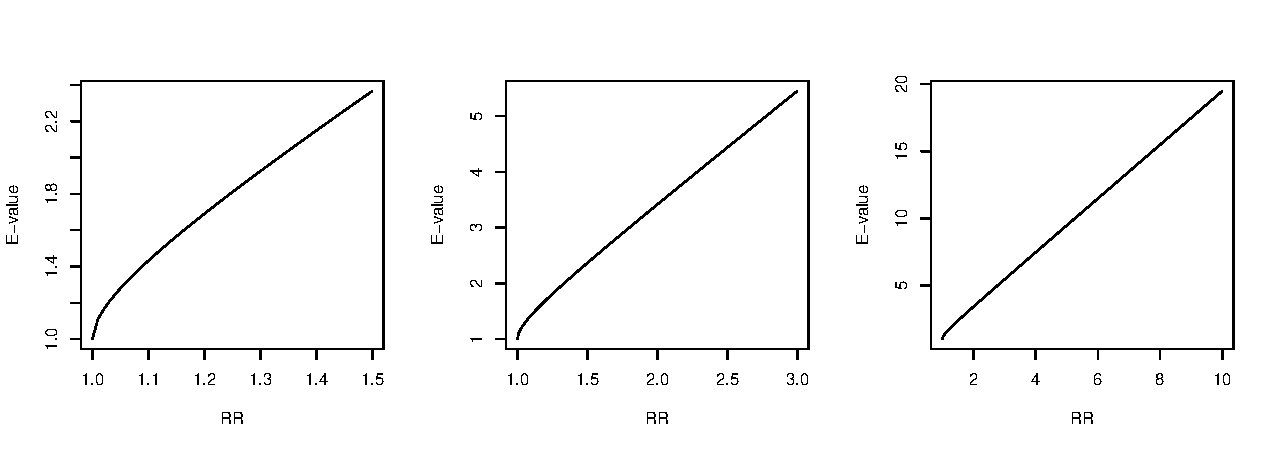
\includegraphics[width=\textwidth]{figures/value_rr.pdf}
\caption{E-value as a monotone transformation of the risk ratio: three figures have different ranges of the risk ratio.}\label{fig::evalue-rr}
\end{figure}

From Figure \ref{fig::evalue-rr}, we can see that if the risk ratio is large, then the E-value $\RR_{ZY\mid x}^\obs + \sqrt{ \RR_{ZY\mid x}^\obs (\RR_{ZY\mid x}^\obs - 1)}$ is nearly $2 \RR_{ZY\mid x}^\obs$ which is linear in the risk ratio. For a small risk ratio, the E-value is more nonlinear in $ \RR_{ZY\mid x}^\obs$. Critics often say that the E-value is merely a monotone transformation of the point estimator or the confidence limits of the risk ratio. So it does not provide any additional information. 


This is partially true. Indeed, the E-value is entirely based on the point estimator or the confidence limits of the risk ratio. However, it has a meaningful interpretation based on Theorem \ref{thm::bounding-factor}: to explain away the observed risk ratio, the maximum of the confounding measures must be at least as large as the E-value. 







%\subsection{E-value is only one-sided}
%
%
%In classic statistics, the $p$-value is often criticized to be one-sided. That is, we reject the null hypothesis with a small $p$-value, but we often do not say that we accept the null hypothesis with a large $p$-value. 
%A large $p$-value may be due to many other reasons, e.g., the sample size is small, the test statistics lack power, etc.
%The E-value has a similar problem. We are more comfortable saying that the causal evidence is weak with a small E-value, but we may be more conservative in claiming strong causal evidence 
%The critiques in some sense apply to all sensitivity analysis techniques in causal inference. 


\subsection{Calibration of the E-value}



The E-value equals the maximum value of the association between the confounder and the treatment and that between the confounder and the outcome to completely explain away an observed association. An obvious problem is that this confounder is fundamentally latent. So it is not trivial to decide whether a certain E-value is large or small. 
Another related problem is that the E-value depends on how many observed covariates $X$ we have controlled for since it quantifies the strength of the residual confounding given $X$. Therefore, E-values across studies are not directly comparable. The E-value provides evidence for causation but this evidence should be assessed carefully based on background knowledge of the problem of interest. 


The following leave-one-covariate-out approach is an intuitive approach to calibrating the E-value. With $X = (X_1, \ldots, X_p)$, we can pretend that the component $X_j$ were not observed and compute the $Z$-$X_j$ and $X_j$-$Y$ risk ratios given other observed covariates $(j=1, \ldots, p)$. These risk ratios provide the range for the confounding measures due to $U$ if we believe that the unmeasured $U$ is not as strong as some of the observed covariates. However, I am not aware of any formal justification for this approach. 



\subsection{It works the best for  a binary outcome and the risk ratio}


Theorem \ref{thm::bounding-factor} works well for a binary outcome and the risk ratio.  \citet{ding2016sensitivity} also proposed sensitivity analysis methods for other causal parameters, including the risk difference for binary outcomes, the mean ratio for non-negative outcomes, and the hazard ratio for survival outcomes. However, they are not as elegant as the E-value for binary outcomes based on the risk ratio. The next chapter will propose a simple sensitivity analysis method for the average causal effect that can include the outcome regression, IPW, and doubly robust estimators in Part \ref{part::observational-studies} as special cases. 





\section{Homework Problems}


\paragraph{A technical lemma for the proof of Theorem \ref{thm::bounding-factor}}
\label{hw::technical-for-evalue-increasing}

Show that 
$$
f(x) = \frac{ax+1}{bx+1}
$$
is increasing in $x$ if $a>b$ and decreasing in $x$ is $a<b$. 


\paragraph{Technical assumption for Theorem \ref{thm::bounding-factor}}
\label{hw::technical-largerthan1}

Revisit the proof of Theorem \ref{thm::bounding-factor}. Assume $Z\ind Y \mid (X, U)$. Show that if $ \RR_{ZU\mid x} > 1$ but $ \RR_{UY\mid x} < 1$, then $\RR_{ZY\mid x}^\obs < 1$. 


Remark: 
This result is intuitive. Condition on $X.$ It says that if the $Z$-$U$ relationship is positive and the $U$-$Y$ relationship is negative, then the $Z$-$Y$ relationship is negative given the conditional independence of $Z$ and $Y$ given $U$. 
Based on this result, if we assume $\RR_{ZY\mid x}^\obs > 1$ and $ \RR_{ZU\mid x} > 1$, then $ \RR_{UY\mid x} > 1$ must be true. 
Therefore, the third condition in \eqref{eq::largerthan1-evalue} is in fact redundant. 



\paragraph{Lemma \ref{lemma::betaw1w2}}\label{hw::proof-lemma-evalue}

Prove Lemma \ref{lemma::betaw1w2}.

\paragraph{\citet{Schlesselman::1978}'s formula}\label{hw::Schlesselman1978formula}

For simplicity, we condition on $X$ implicitly in this problem. 
Consider a binary treatment $Z$, outcome $Y$, and unmeasured confounder $U$.
Assume a common risk ratio of the treatment on the outcome within both $U=0$ and $U=1$:
$$
%\RR_{ZY}^{\true}  =
 \RR_{ZY|U=0} = \RR_{ZY|U=1}, 
$$
and also a common risk ratio of the confounder on the outcome within both $Z=0$ and $Z=1$:
$$  
\RR_{UY|Z=0} = \RR_{UY|Z=1} , \text{ denoted by }\gamma.
$$

Show that  
$$
\frac{\RR_{ZY}^{\obs}}{  \RR_{ZY}^{\true} } = \frac{1 + (  \gamma  -1)\pr(U=1\mid Z=1)  }
{ 1 + (  \gamma -1)\pr(U=1\mid Z=0) } .
$$ 




Remark: First verify that if  $\RR_{ZY|U=0} = \RR_{ZY|U=1}$ then 
$$
\RR_{ZY}^{\true}  = \RR_{ZY|U=0} = \RR_{ZY|U=1} . 
$$
This identity shows the {\it collapsibility} of the risk ratio. 
In epidemiology, the risk ratio is a {\it collapsible} measure of association.


 
\citet{Schlesselman::1978}'s formula does not assume conditional independence $Z\ind Y\mid U$, but assumes homogeneity of the $Z$-$Y$ and $U$-$Y$ risk ratios. It is a classic formula for sensitivity analysis. It is an identity that is simple to implement with pre-specified
$$
\{   \gamma  ,  \pr(U=1\mid Z=1), \pr(U=1\mid Z=0)  \} .
$$
However, it involves more sensitivity parameters than Theorem \ref{thm::bounding-factor}. Even though Theorem \ref{thm::bounding-factor} only gives an inequality, it is not a loose inequality compared to \citet{Schlesselman::1978}'s formula under stronger assumptions. With Theorem \ref{thm::bounding-factor},  \citet{Schlesselman::1978}'s formula is only of historical interest. 



 
\paragraph{E-value after logistic regression: data analysis}\label{hw::eg::NCHS2003}

This problem uses the same dataset as Example \ref{eg::NCHS2003}. 

Report the E-value for the outcome \ri{preeclampsia}. 


\paragraph{Cornfield-type inequalities for the risk difference}\label{hw::cornfield-rd}



Consider binary $Z, Y, U$, and condition on $X$ implicitly. Assume latent ignorability given $U$.  Show that under $Z\ind Y\mid U$, we have
\begin{eqnarray}
\RD_{ZY}^\obs = \RD_{ZU} \times \RD_{UY}
\label{eq::cornfield-rd}
\end{eqnarray}
where $\RD_{ZY}^\obs$ is the observed risk difference of $Z$ on $Y$, and $\RD_{ZU}$ and $ \RD_{UY}$ are the treatment-confounder and confounder-outcome risk differences, respectively (recall the definition of the risk difference in Chapter \ref{sec::twobytwotables-withresume}). 


Remark: Without loss of generality, assume that $\RD_{ZY}^\obs, \RD_{ZU} ,\RD_{UY}$ are all positive. Then \eqref{eq::cornfield-rd} implies that 
$$
\min(\RD_{ZU}  , \RD_{UY}) \geq \RD_{ZY}^\obs
$$
and
$$
\max(\RD_{ZU}  , \RD_{UY}) \geq  \sqrt{ \RD_{ZY}^\obs} .
$$
These are the Cornfield inequalities for the risk difference with a binary confounder.
They show that for an unmeasured confounder to explain away an observed risk difference $\RD_{ZY}^\obs$, the treatment-confounder and confounder-outcome risk differences must both be larger than $\RD_{ZY}^\obs$, and the maximum of them must be larger than the square root of $\RD_{ZY}^\obs$.

\citet{Cornfield::1959} obtained, but did not appreciate the significance of \eqref{eq::cornfield-rd}. \citet{gastwirth1998cornfield} and \citet{poole2010origin} discussed the first Cornfield condition for the risk difference, and \citet{ding2014generalized} discussed the second. 

\citet{ding2014generalized}  also derived more general results without assuming a binary $U$. Unfortunately, the results for a general $U$ are weaker than those above for a binary $U$, that is, the inequalities become looser with more levels of $U$. This motivated \citet{ding2016sensitivity} to focus on the Cornfield inequalities for the risk ratio, which do not deteriorate with more levels of $U$.




\paragraph{Recommended reading}


\citet{ding2016sensitivity}  extended and unified the Cornfield-type sensitivity analysis, which is the theoretical basis for the notion of E-value.   

